Mit der Abnahme des Projektes sind die Ziele des Kunden für den Rahmen des Projektes vollständig erfüllt worden. Es bestehen trotzdem noch Möglichkeiten das System zu erweitern. Ein Punkt wäre das Layout der Website. Die Website beinhaltet zwar das Impressum, aber dies ist aber auf der „About“- oder „Über Uns“-Seite doch sehr versteckt. Man könnte das Impressum beispielsweise in einen Footer verschieben den man auf allen Seiten sehen kann. Ein weiterer Punkt wäre ein Shopsystem. Dafür müssten die nötigen Anpassungen auf den relevanten Seiten getroffen werden, aber auch die Datenbank müsste für diesen Schritt sehr erweitert werden. Noch dazu kommt, dass das Usermanagement momentan sehr rudimentär implementiert ist, was in einer zukünftigen Version etwa aussehen könnte wie in Abbildung \ref{fig:benutzerspeicherung_datenbank}.

%\begin{figure}[h]
%	\centering
%	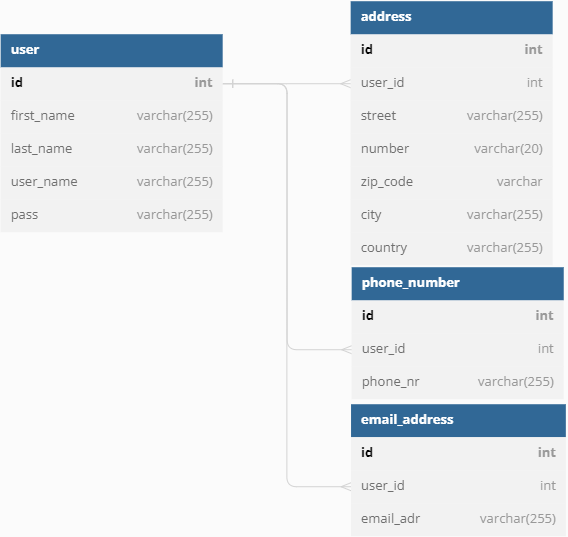
\includegraphics[width=15cm]{images/DatabaseSchemeFuture.png}
%	\caption[Benutzerspeicherung Datenbank]{Benutzerspeicherung in der Datenbank}
%	\label{fig:benutzerspeicherung_datenbank}
%\end{figure}

Der dritte Punkt wäre die Verschlüsselung der Kundendaten. Aktuell wird lediglich das Passwort mit der Methode md5 im Backend, also von Nodejs, gehashed. Das Ziel war ursprünglich alle vom Nutzer eingegebenen Daten im Frontend, also Clientside, zu hashen und zu salten, damit ein potentieller Man-in-the-middle-Angriff sehr viel weniger gefährlich für die Nutzer des Systems und die Optikerkette sind. Man würde durch diese Maßnahme außerdem die Privatsphäre der Nutzer schützen, da keiner der Administratoren die Daten der Nutzer dann willkürlich aus der Datenbank auslesen kann.
